Based on the design principles and problems outlined above, I present my design for an in-\gls{acr:nic}, task-independent, online \gls{acr:rl} system---\emph{\approachshort{} (\approach)}.
At a high level, \approachshort{} is designed to use the auxiliary compute exposed by general SmartNIC devices to offer low-latency online learning, scaling according to available on-chip resources at build time.
Its design is based on meeting the following constraints:
\begin{description}
	\item[Low state-action latency.] \gls{acr:rl} \gls{acr:ddn} applications incur $\mathcal{O}\left(\unit{\milli\second}\right)$ latencies due to a combination of expensive function approximation, batching, state steering, and \gls{acr:pcie} handoffs. Ideally, to keep pace with packet rates upwards of \qty{40}{\giga\bit\per\second} we require inference or state-action latencies around $\mathcal{O}\left(\unit{\nano\second}\right)$ or $\mathcal{O}\left(\unit{\micro\second}\right)$. This would enable fine-grained operation on traffic, particularly latency-sensitive control problems. Where possible, this should correspond to increased throughput to better enable the processing of line-rate traffic.
	
	\item[Effectively employ parallelism.] As discussed in \cref{chap:nets}, SmartNIC devices often contain large numbers of slower cores without \glspl{acr:fpu}. As such, to achieve strong latency or throughput bounds we must employ and design algorithms which are both computationally cheap (forbidding \gls{acr:dnn} backpropagation) and parallelisable. Crucially, this also allows users to scale up or down their resource costs to dedicate as many or few cores as needed to meet desired latency or throughput targets.
	
	\item[Use on-device state without stalling packets.] In spite of the above performance goals, at larger policy sizes it becomes more likely that the inference and update steps of an \gls{acr:rl} algorithm will violate packet or pipeline timing constraints. However, we need access to state from the dataplane to meet our goal of low-latency processing. Thus, an in-\gls{acr:nic} \gls{acr:rl} agent must interact with but not execute on the main packet path.
	
	\item[Reconfigurable.] To simplify deployment as network operators' needs change, an \approachshort{} \gls{acr:rl} agent must be able to be easily repurposed at runtime---i.e., without recompilation and installation of firmware or \gls{acr:fpga} designs. While this includes complete model changes, the most useful aspect would be the ability to swap between online and offline modes of operation to increase decision throughput. Moreover, we aim to make use of the control-plane for easier selection of target flows.
	
	\item[Minimise resource use.] Due to the resource-constrained nature of \gls{acr:pdp} hardware, applications and packet pipelines have highly limited \gls{acr:tcam}-accelerated or other high-speed memory (e.g., $\mathcal{O}\left(\unit{\kibi\byte}\right)$). As such, storing replay buffers is infeasible, as are \gls{acr:rl} algorithms which require such buffers for stable learning. This is amplified when learning a shared policy from several flows concurrently.\sidenote{This consideration has historically been labelled as parallel \gls{acr:rl}~\parencite{DBLP:conf/aamas/GroundsK07}, not to be confused with the multicore/parallel algorithms we are also interested in.}
	
%	\item[High throughput?] Blah blah blah.
%	
%	\item[Several flows?] Blah blah blah.
\end{description}

To meet these constraints, \approachshort{} operates alongside a co-hosted P4 dataplane in a SmartNIC, running asynchronously with respect to the packet forwarding path, with its full interaction model given in \cref{sec:opal-sys-model}.
To achieve both inference and learning I employ fixed-point $Q$ numbers as the main data format, and justify this against data formats in other embedded environments (\cref{sec:opal-data-format}).
Classical \gls{acr:rl} algorithms and function approximation schemes---semi-gradient Sarsa and tile coding (\cref{sec:tile-code,sec:demo-rl-sarsa})---enable learning under the memory and computational constraints of \gls{acr:pdp} hardware. This considers different parallel processing strategies, as well as the conversion to a wait-free algorithm enabled by using $Q$ numbers as the primary data format (\cref{sec:opal-algorithm}).

Bringing \approachshort{} to \gls{acr:pdp} \emph{switches} such as the Tofino would be difficult, if not impossible as they closely match the P4 \gls{acr:psa}, leaving no spare general-purpose compute units.
Taking inspiration from real-time programming, a potential solution might be to divide \gls{acr:rl} processing across several packets (i.e., computing a portion of the preference list each time) until further work would delay outbound transmission.
This would introduce new issues in concurrent access, work splitting, and altered timescales for learning: we leave their treatment to future work.

\subsection{Interaction and system model}\label{sec:opal-sys-model}

\begin{figure}
	\centering
	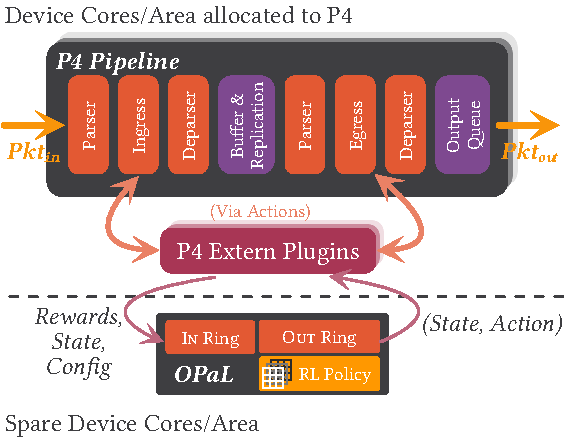
\includegraphics[keepaspectratio, width=0.85\linewidth]{diagrams/opal/arch-with-p4}
	\caption[\approachshort{}'s off-path interaction model with respect to a co-hosted P4 dataplane.]{SmartNIC-type \gls{acr:pdp} devices typically implement a target dataplane design by mapping the processing pipeline across one or more cores or \glspl{acr:fu}. Such devices are well-suited to this; \glspl{acr:npu} or \glspl{acr:soc} such as \glspl{acr:nfp} often have spare cores which aren't dedicated to running the dataplane, while spare area on \glspl{acr:fpga} may be used to design arbitrary \glspl{acr:fu}. While additional compute resources can relax the timing constraints needed to hit line-rate throughput, to prevent packet stalls as required we must move long-running computations (i.e., \gls{acr:rl} inference and updates) to this auxiliary compute. P4 programs expose device-specific functionality through \texttt{extern}s, allowing any extra compute resources and \gls{acr:ipc} to be accessed from ingress and egress tables, thus providing asynchronous execution and fast transmission of P4-extracted state as needed.\label{fig:netro-arch}}
%	\approachshort{} brings low-latency, online reinforcement learning directly to the dataplane. SoC- and NetFPGA-based SmartNIC devices expose spare compute---making in-situ, asynchronous processing and learning possible alongside P4 dataplanes. Classical RL policy methods are the key to making this computationally feasible. ?? REDO
\end{figure}

%?? 
%
%?? need to scale w/ available compute resources.
%
%?? need to not stall.
%
%?? Old, salesman-y.

\approachshort{} is a general, task-independent framework for in-network, online training and execution of \emph{any reinforcement learning agent design} using classical methods.
\approachshort{} is agnostic to the meaning of state vectors it receives as inputs and the actions it produces, which are employed by other functional units or the dataplane.
However, in-\gls{acr:nic} or in-network execution specifically benefits packet-, flow-, and network-level learning, control, and optimisation tasks.
\approachshort{} meets the above goals by operating as a system which exists \emph{in parallel} to a co-hosted P4 dataplane.
\Cref{fig:netro-arch} describes and demonstrates the requisite interaction model; state extraction (i.e., flow telemetry collection and processing) occurs in the ingress and egress \glspl{acr:mat} of the P4 dataplane.
The packet pipeline of a P4 dataplane then communicates with \approachshort{} via \texttt{extern} plugins using \inring{} (state, configuration) messages to reconfigure the agent or request inference, and \outring{} (action) messages which carry output state-action pairs for the environment to make use of.
The contents of these messages are explained below.
To deploy this design, we require a platform-specific implementation of \approachshort{} itself and the \inring{}/\outring{} ring interaction mechanisms---exploiting how SmartNIC devices often expose general-purpose compute.
As many of these devices have engineering and development histories which predate P4, such general compute beyond the P4 \gls{acr:psa}'s limits~\parencite{p4-psa} is surprisingly common.
This then provides path-adjacent, on-chip \gls{acr:rl} in the dataplane.

\approachshort{} itself runs on one or more cores of a SmartNIC to convert state measurements of a known size from the environment into a stream of actions using a stored policy.
I discuss how it scales with additional compute as part of \cref{sec:opal-algorithm}.
%As an example, this might be to map flow state and performance measurements into a queueing priority for future packets from that flow, or to compute and apply a rate limit to preserve quality of service.
These dedicated cores are then responsible for processing requests, computing actions, and updating the underlying policy in real time.
Combined with reward measurements, this policy can then be updated or trained from scratch entirely on the \gls{acr:nic}, acting as a fully online \gls{acr:rl} agent.
An input state vector \emph{always} induces an action and, if online learning is desired, updates the policy using either an included reward or one retrieved from memory according to a key placed alongside the state.
This allows for simultaneous control and learning over independent systems by the same agent (i.e., optimising several flows with their own reward measures, such as \gls{acr:ddos} mitigation in an \gls{acr:as} where each next-hop \gls{acr:as} might have their own health metric).
Configuration messages may be provided over either the data or control-planes, where the P4 control plane may be used to provide access control over which machines or ports may send such commands.

%?? How does this meet the above requirements?
By executing on spare compute units, this design prevents packet stalling by moving longer-running compute out of the packet path, and can scale with cores made available at compile-time to improve latency and throughput.
By operating as closely as possible to the P4 pipeline, \approachshort{} uses and learns from per-packet state with minimal added latency (avoiding \gls{acr:pcie} transfers and batching as required), while imposing minimal impact on carried traffic for both bump-in-the-wire deployments and at end-points.
Moreover, the presence of the P4 dataplane allows easier inclusion of existing P4 traffic measurement and state extraction techniques, such as those covered in \cref{chap:nets}.


%unused device resources beyond the P4-PSA spec \emph{can and should be used} to drive asynchronous environmental control

%\Cref{fig:netro-arch,fig:single-and-parallel} outline our design and implementation on Netronome SmartNIC hardware in pursuit of this goal: unused device resources beyond the P4-PSA spec \emph{can and should be used} to drive asynchronous environmental control.
%We explain relevant NFP architectural details later in \cref{sec:netronome-platform-fundamentals}.
%\approachshort{} communicates with the packet pipeline of a P4 dataplane via \texttt{extern} plugins using \inring{} (state, configuration) and \outring{} (action) messages (\cref{fig:netro-arch}).
%Internally, \approachshort{} either has all its cores act independently (\cref{fig:single-and-parallel:single}) or cooperate to solve each task (\cref{fig:single-and-parallel:parallel})---with different latency-throughput benefits (\cref{sec:action-and-update-computation}).
%We open-source our firmware and control programs for the benefit of the community.
%Moving beyond the Netronome platform, we describe how our architecture may be adapted and improved on by bespoke hardware or FPGA-based deployment.

%However, high-speed data networks impose inviolable per-packet deadlines.

%To protect traffic throughput and allow effective deployment in as many environments as possible, \approachshort{} places RL execution on-chip, \emph{but off the main packet path}, communicating and running parallel to the main P4 dataplane.
%As shown in \cref{fig:netro-arch}, this asynchrony allows coexistence with P4 programs, and imposes minimal impact on carried traffic for both bump-in-the-wire deployments and at end-points.
%For instance, in the default deployment of a P4 packet processing pipeline on Netronome NFP chips several cores go unused (as does spare area on an FPGA design), making this paradigm possible.

\paragraph{Execution trace handling.}
To be generally applicable, we require that \approachshort{} is flexible in how reward values are mapped to input state vectors.
Target applications may aim to control one or many separate trajectories---i.e., learning from concurrent traces~\parencite{DBLP:conf/aamas/GroundsK07}---and in the online case we must have a low-overhead method of retrieving the correct last state-action-value tuple.
Moreover, each may require its own reward value depending on the nature of the \gls{acr:mdp}, for instance when optimising individual flow behaviour rather than joint control to benefit a shared environment.
\approachshort{} thus allows several sources for selecting these values, which may be configured separately for trace and reward selection:
\begin{description}
	\item[Shared.] A single \gls{acr:rl} trajectory or reward value is held. The reward value must be periodically updated using dedicated reward packets.
	\item[Field.] A given field of the input state vector is used as the lookup key (e.g., in a hash table) for either the trajectory or reward value. For instance, this may be a packet's flow hash or source \gls{acr:ip}. The reward value must be periodically updated as above.
	\item[Raw Field.] A given field of the input state vector is used as in \emph{Field}, but is not hashed for lookup.
	\item[Value.] A given field of the input state vector is directly used as the reward value. The installed policy can use or ignore this field as needed.
\end{description}

\paragraph{Policy constraints.}
To minimise (and predetermine) the amount of data required to encode a policy, as well as reduce the computational complexity of policy inference, tile coded policies are constrained in the following ways.
All tilings are assumed to be uniform rectilinear grids as in \cref{alg:tile-code}, where each dimension of input state has a single minimum and maximum assigned.
We assume that each dimension is subdivided into the same number of tiles, and that all tiling sets contain the same number of overlapping tilings over a given list of dimensions.
Each tiling set then covers a list of dimensions up to a platform-defined size.

\paragraph{Message formats.}
To provide the needed functionality and runtime configuration, \approachshort{}'s \inring{} ring receives the following message types.
\begin{description}
	\item[State messages.] These contain only a list of input data values from the environment, which invokes an inference and/or update cycle.
	\item[Reward messages.] These contain a single data value, and an optional data value used as a key to ensure it is mapped to the correct state trajectory.
	\item[Configuration.] These messages contain either top-level parameters (action counts, dimension counts, hyperparameters), or the dimension list for each tiling set.
	\item[Policy insertion.] As network packets have a restricted size, these messages subdivide a full policy parameter vector, and contain an array of tile value data alongside an \emph{offset} into the policy. These may be used to insert a pretrained policy into an offline agent, or to percolate policy updates among online learning agents in a network.
\end{description}
\approachshort{}'s \outring{} ring only carries a single message class, which is a state-action tuple.

%\begin{figure}
%	\centering
%\resizebox{0.48\linewidth}{!}{\begin{minted}{rust}
%type Tile = i32; /* or i16, or i8. */
%pub enum CtlMsg {
%    State(Vec<Tile>),
%    Reward(Tile),
%    Config(Config),
%    Insert{
%        offset: usize,
%        data: Vec<Tile>
%    },
%}
%
%pub enum Config {
%    Setup { .. },
%    Tiles { .. },
%}
%\end{minted}}
%\resizebox{0.48\linewidth}{!}{\begin{minted}{rust}
%type Tile = i32;
%pub enum CtlMsg {
%	State(Vec<Tile>),
%	Reward(Tile),
%	Config(Config),
%	Insert{
%		offset: usize,
%		data: Vec<Tile>
%	},
%}
%	
%pub enum Config {
%	Setup { .. },
%	Tiles { .. },
%}
%\end{minted}}
%	\caption[Sourec deo]{text}
%\end{figure}

\subsection{Data format}\label{sec:opal-data-format}
%?? data format selection vs alternatives
To implement online learning such as in \gls{acr:rl}, we require a data type which allows us to perform numerical computation without an \gls{acr:fpu}---principally, to compute the values in action preference lists.
Moreover, to achieve online learning we require a format which is both fast to work with (to minimise processing latencies), and suited to represent gradients and temporal difference values, i.e., incremental changes to stored policy weights.
Recalling the discussion in \cref{sec:numerical-representations-for-embedded-ml}, we employ \emph{fixed-point arithmetic}; it offers both the versatility needed to be easily reconfigurable, and it maps simply to \gls{acr:alu} operations.
For instance, only multiplications and additions require additional bitshifts for base pre-/post-conversion, while additions and subtractions require no additional overhead.\sidenote{Depending on the system design, (hyper-)parameters used only in divisions can be replaced with right bitshifts if we restrict their allowed values to negative powers of 2. This comes at the cost of system flexibility, and as such \approachshort{}'s implementation doesn't make use of this possibility.}

%?? Hence not binarised repr.
%?? Can choose bits allocated to fraction at runtime, overall bits at compile.
%?? Mention memory benefits.

From a configurability perspective, the count of fractional bits in a $Q$ number can be easily changed at runtime.
Naturally, this has no effect on overall latency and throughput of fixed-point arithmetic, but is a useful characteristic for being able to deploy different \gls{acr:rl} agents to the same hardware without invoking more costly firmware or \gls{acr:fpga} design installation.
If this is fixed at the same setting for all values used, then we needn't tag individual $Q$ numbers with information about their base, saving memory.
The bit width of the numbers themselves (i.e., $k$) may be changed only at compile time in many cases, particularly as SmartNICs often lack dynamic memory management in their native non-P4 programming environments.
Lower choices of $k$ sacrifice numeric range, but allow policies and data to occupy less memory---allowing fairer resource use versus other dataplane programs---and thus occupy less memory bandwidth in data transfers.
Alternatively, larger policies may be stored in the same memory bounds (potentially enabling the solution of more complex problems).

The reduced width and precision floating-point data formats we also examined earlier are not suitable here, in spite of their successes in other embedded domains.
First and foremost, these still require specialised \gls{acr:fpu} implementations.
This is naturally at odds with the design and goals of \gls{acr:pdp} hardware, and beyond \gls{acr:fpga} designs such a data format would be infeasible.
Software floating-point emulation has historically required \qtyrange{10}{30}{\times} more cycles to perform compared to hardware \glspl{acr:fpu}~\parencite{DBLP:conf/arith/IordacheT03}, which is incompatible with our need for low-latency and high-throughput processing.
While the added dynamic range would be useful in this application, performance is a primary goal.

\gls{acr:pdp} hardware excels in applying actions to network packets using \glspl{acr:mat}, potentially giving us a high-performance method to install selected actions within the network.
However, directly modifying these match tables from within the device itself is neither feasible nor safe.
On Netronome \gls{acr:nfp} hardware in particular, rule updates \emph{must} be applied by the co-hosted controller machine, as tables are reliant on the optimised DCFL~\parencite{DBLP:conf/infocom/TaylorT05} data format.
In addition to the prohibitive complexity of building this data structure on-device, its construction requires knowledge of the entire rule set (and cannot be incrementally updated).
I instead suggest in general that \texttt{extern}s or datapath stages which apply \gls{acr:rl} actions to packets should maintain a small store of state-action pairs, and periodically send these back to the controller for batch installation.
This ensures that the majority of installed rules benefit from faster hardware-accelerated lookups, while preventing installation delay on the newest decisions.
Platforms such as Intel Tofino greatly simplify this, where Tofino Native Architecture intrinsics such as \emph{Action Profiles/Selects} allow a P4 action to be chosen based on a register value (e.g., an \gls{acr:rl} action).
Future \glspl{acr:nic} and SmartNICs may expose support for runtime table modification via the Portable \gls{acr:nic} Architecture~\parencite{p4-pna} as discussed in \cref{sec:frontiers-in-programmable-networks}, but at present these proposals are under constant revision and are far too nascent to seriously consider.

\subsection{Algorithm}\label{sec:opal-algorithm}
To enable online in-\gls{acr:nic} learning in spite of the computational limits of \gls{acr:pdp} hardware, we must return to \emph{classical} \gls{acr:rl} methods and models.
In particular, we focus on tile coding with one-step temporal-difference learning algorithms such as Sarsa, which were discussed and explained earlier (\cref{sec:tile-code} and \cref{sec:demo-rl-sarsa}).
%These choices have important benefits for in-NIC execution.
These functions do not require batches of inputs to learn in a stable way, negating the memory needed to store experience replays, and have simple update and inference logic.
Moreover, gradient computation is identical to the forward pass and has no dependency on the current parameter values $\wvec{}$, potentially allowing hit tiles to be stored to accelerate the next update step.
Finally, the choice of single-step algorithms (as opposed to $n$-step or Monte Carlo methods) bounds the amount of per-trace state required for online learning to just the last state-action pair, safeguarding the limited memory of our target devices.

As for how to take advantage of the multicore nature of SmartNICs, there are two strategies worth considering.
Suppose we have $n$ cores.
The first strategy is that we simply have each core work independently.
For instance, when dealing with a stream of input state vectors according to \approachshort{}'s interaction model, we may serve each arrived vector to a free core---this core then tile codes the state against every tiling, produces an output action, and then updates the policy as required (\cref{alg:tile-code,eqn:sg-sarsa}).
Intuitively, this produces an $n$~\unit{\times} throughput improvement assuming there are no bottlenecks at either the input and output queues or mutual exclusion around shared data.
However, this offers no reduction to the processing time of any \emph{individual} element---and so the state-action latency is not reduced as desired.

\begin{figure}
	\centering
	\resizebox{0.67\linewidth}{!}{
		\begin{tikzpicture}
	\node at (0,0) {
		\begin{tikzpicture}
			\draw[step=0.5cm,color=uofgcobalt,opacity=0.7,shift={(0,0)},label=above:{Tiling 0}] (-0.5,-0.5) grid (1,1);
			\fill[uofgcobalt,opacity=0.5] (0.5,-0.5) rectangle (1,0);
			\node[color=uofgcobalt] (t1g) at (0,1.2) {\footnotesize Tiling 1};
			
			\draw[step=0.5cm,color=uofgpumpkin,opacity=0.9,shift={(0.25,-0.25)},label=above:{Tiling 1}] (-0.5,-0.5) grid (1,1);
			\fill[uofgpumpkin,opacity=0.5,shift={(0.25,-0.25)}] (0,0) rectangle (0.5,0.5);
			\node[color=uofgpumpkin!50!uofgrust] (t2g) at (0.25,-0.95) {\footnotesize Tiling 2};
			
			\node[circle, black, draw,
			fill, radius=0.5pt, inner sep=0pt,minimum size=1.5pt, label=above:{$s$}] at (0.625,-0.125) {};
			%			\filldraw (0.625,-0.125) circle[radius=1.5pt,label=above:{$s$}];
			
			\draw[->] (-0.25,-0.5)--(-0.25,0.85);
			\draw[->] (-0.25,-0.5)--(1.1,-0.5);
			
			\node at (1,-0.7) {\footnotesize 1};
			\node at (-0.4,0.75) {\footnotesize 1};
			\node at (-0.35,-0.6) {\footnotesize 0};
		\end{tikzpicture}
	};
	
	\node (policy-head) at (2.5,1.2) {Policy};
	\draw[color=uofgcobalt,opacity=0.7] (2,0) rectangle ++(2,1) node[pos=.5] (t1p) {Tiling 1};
	\fill[uofgcobalt,opacity=0.25] (3.33,0) rectangle ++(0.67,0.33);
	
	\draw[color=uofgpumpkin,opacity=0.9] (2,-1) rectangle ++(2,1) node[pos=.5] (t2p) {Tiling 2};
	\fill[uofgpumpkin,opacity=0.25] (2.67,-0.67) rectangle ++(0.67,0.33);
	
	\draw (2,-2) rectangle ++(2,1) node[pos=.5] (tdot) {$\cdots$};
	
	\draw [->,color=uofgcobalt, bend left] (t1g) to (t1p.west);
	\draw [->,color=uofgpumpkin, bend right] (t2g) to (t2p.west);
	
	\node (act-list) at (1,-2.5) {$\mathbf{a}=\left[ \cdots \right]$};
	
	\draw [->, bend right] (t1p.west) to (act-list);
	\draw [->, bend right] (t2p.west) to (act-list);
	\draw [->, bend right] (tdot.west) to (act-list);
\end{tikzpicture}
	}
	\caption[A visualisation of how tile-coding can be split into subtasks as a map-reduce problem.]{Tile-coded function approximation can be considered as a map-reduce problem during both the inference and update steps. Action preferences are aggregated from \emph{disjoint} tile queries, where each tile hit contains a list of action values to add to $\mathbf{a}$. Retrieving or updating each tiling is thus a separate task. As all constituent action preference lists are disjoint between tasks, updating hit tiles requires no control over concurrent accesses---furthermore, it requires no final aggregation step.\label{fig:opal-par-tilecode}}
\end{figure}

To attain the latency improvements we desire, we must consider instead a second strategy: how several cores may work together to complete an individual inference or update operation.
Consider that tile coding computes individual hits against a set of tilings to produce a sparse boolean feature vector, which we'll denote $\mathbf{x}$, and refer to the set of all its non-zero indices by $H$.
Without loss of generality, suppose we have two tilings $t_1$ and $t_2$, with a number of tiles $|t_1|$ and $|t_2|$ in each respectively (such that $\dim{\mathbf{x}}=|t_1|+|t_2|$).
For notational simplicity, let each entry of an agent's policy data $\wvec{}$ be a vector of length $A$ (i.e., choosing between $A$ discrete actions).
A state vector will produce exactly one hit in each tiling, having indices $h_1\in[0,|t_1|)$ and $h_2\in[|t_1|,|t_1|+|t_2|)$, without overlap.
The final action preference list is given by \cref{eqn:lin-approx}, which we can specialise further:
$$
\mathbf{a} = \wvec{}^{\top} \mathbf{x} = \wvec{}\left[h_1\right] + \wvec{}\left[h_2\right] = \sum_{h\in{}H}\wvec{}\left[h\right]
$$
As a result, tile coded \gls{acr:rl} inference may be subdivided into several distinct computations of tile indices whose results are added together as a final aggregation step.
Most of the work in each task arises from computing the tile index hit by the state vector.
Crucially, we have shown that memory regions of each tiling have no overlap with one another by construction.
Each memory address is visited and owned by exactly one task---hence, there is no concurrent access to policy values---and so no locks are required to protect each region of the policy.
\Cref{fig:opal-par-tilecode} demonstrates this process visually.

When updating the policy we need only monitor the number of completed tasks rather than perform a final aggregation step.
To see this, we specialise Sarsa's update step (\cref{eqn:sg-sarsa-update}) using our list of hit indices $H$.
After centrally computing a \gls{acr:td} value $\delta_t$ using $\mathbf{x}$ and a subsequent $\mathbf{x}'$, the action $a$ invoked by $\mathbf{x}$, and a learning rate $\alpha$, we update the policy values involved in the previous decision (using Python slice notation for simplicity):
\begin{align*}
\wvec{}\left[:,a\right] := \wvec{}\left[:,a\right] + \alpha\delta_t \mathbf{x}\\
\therefore~\wvec{}\left[h_1,a\right] := \wvec{}\left[h_1,a\right] + \alpha\delta_t,\\
\therefore~\wvec{}\left[h_2,a\right] := \wvec{}\left[h_2,a\right] + \alpha\delta_t.
\end{align*}
and so on for all $h \in H$ when we have an arbitrary number of tilings.
Thus, using the above knowledge that concurrent accesses to any parts of the policy cannot occur, an \gls{acr:rl} update divides into subtasks without locking in much the same fashion as inference does.

The aggregation step still risks becoming a bottleneck during inference; if individual preference lists are passed back as discrete messages, then this requires explicitly iterating over and summing all such lists.
While this may be performed by a dedicated worker thread or core in parallel to the other disaggregated inference tasks, this involves additional costs in every such task for \texttt{memcpy} operations into a message buffer.
Consider again that \approachshort{} targets \gls{acr:pdp} hardware: without a dynamic memory allocator, this buffer has bounded length and so risks causing head-of-line blocking for all other tasks.
However, encoding our values using a fixed-point representation allows us to employ atomic instructions to remove the aggregate step, thus producing a wait-free algorithm.
Recall that the aggregation step involves \emph{only additions}, that atomic integer fetch-add instructions are commonly offered on many machine architectures,\sidenote{While other datatypes such as \mintinline{rust}{f32} can technically support atomic operations on many platforms, outside of specialised \gls{acr:gpu} environments such as CUDA these incur non-trivial performance costs due to cache and register placement restrictions.} and that fixed-point addition is identical to integer addition.
As a result, the final action preference list may be allocated once and atomically added to by all workers.
Moreover, if extra care is required to prevent numeric overflows or ensure saturation, then any worker may locally verify whether the fetched value and summand would cause an overflow.
Alternately, an implementer may simply enforce upper and lower bounds on each action value to prevent positive or negative overflow.

\begin{algorithm}
	\caption{ParSa---\emph{Par}allel \emph{Sa}rsa\label{alg:parsa}}
	\SetKw{Let}{let}
	\SetKw{Enum}{enum}
	\SetKw{In}{in}
	\SetKw{Await}{await}
	\SetKw{Const}{const}
	\SetKwProg{parsa}{Function \emph{ParSa}}{}{end}
	\SetKwProg{control}{Function \emph{Ctl}}{}{end}
	\SetKwProg{minion}{Function \emph{Minion}}{}{end}
	\SetKwProg{tilecode}{Function \emph{TileCode}}{}{end}
	
	\tcc{Given message passing mechanisms \emph{scatter} and \emph{recv}, an input request stream \inring{}, an output action stream \outring{}, quantised arithmetic functions $Q_\mathit{mul}$ and TileCode, and omitting schedule/config/precache/reward updates.}
	\tcc{\emph{cfg}.$\alpha$, \emph{cfg}.$\gamma$ are hyperparameters affecting the significance of each update and the degree of forward-planning, respectively.}
	
	\Enum Par \{ Act(\emph{state}), Upd(\emph{delta, action, state}) \}\;
	\Const \emph{cfg, policy} = /* ... */\;
	
	\Let \emph{values}: [AtomicI32; \emph{cfg.n\_actions}] = \{0\}\;
	\Let \emph{acks}: AtomicI32 = 0\;
	\parsa{id, schedule}{\label{alg:parsa:par}
		\uIf{id==0}{\label{alg:parsa:parctl-start}
			\ForAll{state\_pkt \In \inring{}}{
				Ctl(\emph{state\_pkt})\;
			}
		}\label{alg:parsa:parctl-end}
		\Else{\label{alg:parsa:parminion-start}
			\While{true}{Minion(\emph{schedule}[$\mathit{id}- 1$], recv())\;}
		}\label{alg:parsa:parminion-end}
	}

	\control{state}{\label{alg:parsa:parctl-begin}
		\emph{values, acks} = \{0\}, scatter(Par::Act(\emph{state}))\;\label{alg:parsa:parctl-act}
		acquire slot for \outring, copy \emph{state} into slot\;\label{alg:parsa:parctl-preprep}
		\Await acks == \emph{cfg.n\_minions}\;\label{alg:parsa:parctl-await1}
		\Let \emph{action} = argmax(\emph{values})\;\label{alg:parsa:parctl-acchoose}
		write \emph{action} into \outring{} slot, enqueue\;\label{alg:parsa:parctl-acemit}
		\If{cfg.online}{
			\Let \emph{((l\_state, l\_act, l\_val), found\_s)} = \emph{cfg}.lookup\_state\_from\_key(\emph{state})\;\label{alg:parsa:parctl-checkstate}
			\Let \emph{(reward, found\_r)} = \emph{cfg}.lookup\_reward\_from\_key(\emph{state})\;\label{alg:parsa:parctl-checkreward}
			\If{found\_s \&\& found\_r}{
				\Let $\delta_t$ = $\mathit{reward} + Q_\mathit{mul}$(\emph{cfg}.$\gamma$, \emph{values}[\emph{action}]) $-$ \emph{l\_val}\;\label{alg:parsa:parctl-td1}
				$\delta_t$ = $Q_\mathit{mul}$(\emph{cfg}.$\alpha$, $\delta_t$)\;\label{alg:parsa:parctl-td2}
				\emph{acks} = 0, scatter(Par::Upd($\delta_t$, \emph{l\_act}, \emph{l\_state}))\;\label{alg:parsa:parctl-update}
				\Await acks == \emph{cfg.n\_minions}\;\label{alg:parsa:parctl-await2}
			}
			\emph{cfg}.store\_state(\emph{state}, \emph{action}, \emph{values}[\emph{action}])\;\label{alg:parsa:parctl-store}
		}
	}

	\minion{tasks, msg}{
		\Switch{msg}{
		\uCase{Par::Act(\emph{s})}{
			\ForAll{task \In tasks}{
				\Let \emph{hit} = TileCode(\emph{s}, \emph{task})\;\label{alg:parsa:parminion-acthit}
				\For{i \In [0..cfg.n\_actions)}{\label{alg:parsa:parminion-liststart}
					\emph{values}[\emph{i}].atomic\_add(\emph{policy}[\emph{hit}][\emph{i}])\;
				}\label{alg:parsa:parminion-listend}
			}
		}
		\uCase{Par::Upd($\delta$, \emph{a}, \emph{s})}{
			\ForAll{task \In tasks}{
				\Let \emph{hit} = TileCode(\emph{s}, \emph{task})\;\label{alg:parsa:parminion-acthit2}
				\emph{policy}[\emph{hit}][\emph{a}] += $\delta$\; \label{alg:parsa:parminion-update}
			}
		}
		}
		\emph{acks}.atomic\_add(1)\;\label{alg:parsa:parminion-lastack}
	}

%	\tilecode{state, task}{
%		\Let \emph{hit} = \emph{cfg}.get\_task(task)\;
%	}
\end{algorithm}

Parallelising the \gls{acr:rl} algorithm among processes in this way thus requires tight coupling between the function approximation and \gls{acr:rl} update algorithm.
The combination of all of these elements forms the basis of \emph{ParSa}---parallel Sarsa (\cref{alg:parsa}).
To match the deployment environment of SmartNIC devices, ParSa is presented such that each worker thread operates in an infinite loop to await and process requests delivered over a message channel \inring{}, and produce a stream of outputs on \outring{}.
We first assume that every process knows its own index---\emph{id}---and that a \emph{schedule} has been precomputed to divide individual tilings among cores as tasks (\cref{alg:parsa:par}).
This careful division is important; an individual tiling may contain several dimensions, and by recalling \cref{alg:tile-code} it is obvious that tilings with a higher dimension count require more iterations and are thus more expensive to infer.
To give some context on the number of tasks ParSa is expected to perform, a policy sized to match the agent designs from \cref{chap:ddos-rl} with one bias tile and \num{16} sets of \num{8} tilings creates \num{129} work items.
As such, a schedule is required to produce the most balanced workload between worker threads.\sidenote{Work stealing or other parallelisation strategies are not suitable choices for work balancing in tile coded Sarsa for several reasons. These include the computational simplicity of individual tasks, the predictable compute cost of any such task, and the relative cost of \gls{acr:ipc} required to pass cached state between workers.}
However, this is a deployment-specific implementation detail, as in addition to raw task costs an effective scheduler must account for cache size limits and physical/logical core differences.
I present an allocator tailored to Netronome hardware later in \cref{alg:parsa-schedule}.
A single worker thread, designated as the \emph{controller}, then receives and processes state vectors from the environment (\crefrange{alg:parsa:parctl-start}{alg:parsa:parctl-end}), while the remaining threads---\emph{minions}---retrieve a broadcast message of type \emph{Par} to apply over their prescheduled task set (\crefrange{alg:parsa:parminion-start}{alg:parsa:parminion-end}).

The \emph{Ctl} procedure directs tasks to minion threads, manages storage of execution traces, and computes the policy adjustments prescribed by the Sarsa \gls{acr:td} value.
Applying the insights of \textcite{DBLP:journals/firai/TravnikMSP18} to minimise action latency, an action is computed and sent out into the environment---and only then is the underlying policy updated.
For each input state, the controller thread zeroes out the shared aggregation space, where \emph{values} holds the aggregated action preference list and \emph{acks} contains the count of terminated minion threads.
An \emph{Act} request is then sent as a broadcast message to all minion threads using the platform-specific \emph{scatter} \gls{acr:ipc} call (\cref{alg:parsa:parctl-act}).
While the minions produce the action preference list asynchronously, the control thread then requests an output message slot and prepares it by copying the state into the acquired buffer (\cref{alg:parsa:parctl-preprep}).\sidenote{In principle, the controller thread may also act as another minion after this step, between scatter and recv calls, subject to code store limits.}
Once every thread has marked its termination, the values of each action given the input state are located in \emph{values} (\cref{alg:parsa:parctl-await1}).
The index of the largest value is then taken to be the chosen action, though this may be trivially modified to account for $\epsilon$-greedy selection (\cref{alg:parsa:parctl-acchoose}), which is then placed into the output message and returned to the environment (\cref{alg:parsa:parctl-acemit}).
When online learning is enabled, the control thread checks for a reward signal and prior state-action-value tuple according to the configured trace selection scheme from \cref{sec:opal-sys-model} (\crefrange{alg:parsa:parctl-checkstate}{alg:parsa:parctl-checkreward}).
If a match is found, it computes and reduces by $\alpha$ the Sarsa \gls{acr:td} value $\delta_t$ (\crefrange{alg:parsa:parctl-td1}{alg:parsa:parctl-td2}), before passing this adjustment and the prior state action pair to the minion threads to perform the update step (\crefrange{alg:parsa:parctl-update}{alg:parsa:parctl-await2}).
Modification to other single-step algorithms such as \emph{Q-learning} would be simple, requiring only changes to the computation of $\delta_t$.
The newest state-action-value tuple is then stored (\cref{alg:parsa:parctl-store}).

The \emph{Minion} procedure processes a single request to retrieve and aggregate, or update, the action values learnt for an input state over some subset of the policy tilings, \emph{tasks}.
All minion threads cover the complete set of tilings between themselves.
In the case that action inference is requested, the policy hit index is computed against the input state for each tiling in this thread's task list (\cref{alg:parsa:parminion-acthit}).
As described above, each action value is atomically added to its matching position in the shared preference list \emph{values} (\crefrange{alg:parsa:parminion-liststart}{alg:parsa:parminion-listend}).
When an update is requested, all tile hit indices are recomputed (\cref{alg:parsa:parminion-acthit2}), and an adjustment $\delta$ is added to the selected action in each case (\cref{alg:parsa:parminion-update}).
Once all subtasks have been completed, this thread's completion is recorded (\cref{alg:parsa:parminion-lastack}).
While it is apparent that the indices of hit tiles may also be locklessly sent back and stored as part of the execution trace---i.e., by adding an extra value slot per task---the number of subtasks often far exceeds the count of values in a state vector.
As a result, this results in a larger \texttt{memcpy} in \emph{Ctl} (the serial portion of ParSa), and as such it is more efficient to recompute hit indices in the update step---though this optimisation is useful in the case of the first (non-ParSa) parallelisation strategy.

%?? mention that theoretical worse than just adding more cores due to message passing costs, memfence, compiler reordering etc., size of serial portion, number of constituent tasks. (could split to indiv actions, but need stupid cores for feasible.)
As required, this new algorithm scales with increasing processor counts to reduce both the inference and update costs incurred by a single state vector.
This lowers the state-action latency and produces a corresponding increase to throughput.
However, the factor of speedup is \emph{worse} than $n$~\unit{\times}, and exhibits diminishing returns in terms of core count---for instance due to the cost of \texttt{memcpy}s and arithmetic in the serial logic of \emph{Ctl}, message passing costs at the broadcast and receive steps, and any memory fences or reorderings inserted by the compiler around atomic arithmetic.
This is limited further by the number of subtasks which can be generated for a given policy.
While ParSa assumes tile-level granularity, it may be modified to compute individual actions at the cost of being dominated by significant repetition of work and \gls{acr:ipc} overheads.
Since these aspects are platform-dependent, this behaviour can only be shown empirically as in \cref{sec:opal-results-work-alloc}.